\documentclass{beamer}

% Set up
\usepackage{xcolor}
\usepackage{graphicx}
\usepackage{amsmath}
\usepackage{graphicx}
\usepackage{amsthm}
\usepackage{mathrsfs}  
\usepackage{amsfonts}
\usepackage{amssymb}
\usepackage{amsmath}
% \usepackage[utf8]{inputenc}

% Beamer setup
\usetheme{default}
\usecolortheme{default}
% \AtBeginSection[]
% {
%   \begin{frame}
%     \frametitle{Table of Contents}
%     \tableofcontents[currentsection]
%   \end{frame}
% }
\usefonttheme[onlymath]{serif}

% Math commands
\newcommand{\1}{\mathbbm{1}}
% measures / sets of measures:
\newcommand{\mH}{\mathscr{H}}
\newcommand{\mL}{\mathscr{L}}
\newcommand{\mP}{\mathscr{P}}
\newcommand{\cH}{\mathcal{H}} % entropy
\newcommand{\cT}{\mathcal{T}} % topology
\newcommand{\cB}{\mathcal{B}} % borel
\newcommand{\W}{\mathcal{W}} % new metric W
\newcommand{\X}{\mathcal{X}} % space X
\newcommand{\nabladot}{\nabla\cdot} % discrete divergence operator
\newcommand{\A}{\mathcal{A}} % action
\newcommand*\de{\mathop{}\!\mathrm{d}}
\DeclareMathOperator*{\argmin}{arg\,min}
\DeclareMathOperator*{\argmax}{arg\,max}
\DeclareMathOperator*{\supp}{supp}
\DeclareMathOperator*{\id}{id}
\DeclareMathOperator{\imm}{Im}
\DeclareMathOperator{\lalpha}{\overline{\alpha}}
\DeclareMathOperator{\aconv}{\alpha \textit{x}+\overline{\alpha}\textit{y}}
\DeclareMathOperator{\bconv}{\beta \textit{x}+\overline{\beta}\textit{y}}

%%%%%%%%%%%%%%%%%%%% from the paper
\newcommand{\R}{\ensuremath{\mathbb{R}}}
\newcommand{\Z}{\ensuremath{\mathbb{Z}}}
\DeclareMathOperator{\Ric}{Ric}
\DeclareMathOperator{\vol}{vol}

\def\diam{\mathop{\mathrm{diam}}\nolimits}
\def\vol{\mathop{\mathrm{vol}}\nolimits}
\def\area{\mathop{\mathrm{area}}\nolimits}
\def\Hess{\mathop{\mathrm{Hess}}\nolimits}
\def\supp{\mathop{\mathrm{supp}}\nolimits}
\def\Ric{\mathop{\mathrm{Ric}}\nolimits}
\def\Id{\mathop{\mathrm{Id}}\nolimits}
\def\tr{\mathop{\mathrm{tr}}\nolimits}
\def\ac{\mathop{\mathrm{ac}}\nolimits}
\def\div{\mathop{\mathrm{div}}\nolimits}
%%%%%%%%%%%%%%%%%%%%%%%%%%%%%%%%%%%%



%Information to be included in the title page:
\title[Ricci curvature of finite Markov chains]{Ricci curvature of finite Markov chains \\ via convexity of the entropy \\~\\ \small M. Erbar and J. Maas} 
\author[Matilde Dolfato]{\small Matilde Dolfato \\ Mentor: Prof. Elia Brué}
\institute[]{Università Bocconi  \par Visiting Student Initiative - BIDSA}
\date{\today}

\begin{document}


\frame{\titlepage}
%  COMMENT:

% draw on blackboard the 3 macro areas: RICCI CURV, MARKOV CHAINS, OPTIMAL TRANSPORT
% the aim of this paper is to define a notion of ricci curvature lower bound for discrete spaces of markov chains. 
% think of ricci curvature as just a specific way of characterizing the curvature of our space
% having a lower bound on ricci gives results on the convergence of the chain, which are interesting statistically speaking 
% % STUDY
% the notion is differentiable -> can not apply -> uses equivalent notion based on optimal transport (metric notion)

\begin{frame}
\frametitle{Overview}
\tableofcontents
\end{frame}

\section{Introduction}
\tableofcontents[currentsection]
\begin{frame}{What we are talking about}
RICCI CURVATURE\\~\\
\begin{center}
    OPTIMAL TRANSPORT 
\begin{itemize}
        \item \small Wasserstein geometry
        \item \small Convexity of Shannon's entropy
        % \item \small Gradient flow of Shannon's entropy
\end{itemize}
\end{center}~\\
\hfill MARKOV CHAINS

% Piccolo cheat
\color{white}\cite{brue}\cite{lee2018riemann}\cite{lee2003smooth}\cite{lott2009ricci}\cite{Ohta_2014}\cite{villani2008optimal}\cite{maas}\cite{olliviervillani}\cite{ollivier2009ricci}
\end{frame}

\begin{frame}{General theoretical framework}

The heat flow is the gradient flow of the entropy \only<1>{\textcolor{blue}}{in the \(W_{2}\) space}
\\~\\

$\Ric\ge\kappa \Longleftrightarrow \kappa$-convexity of the entropy
    $\Longleftrightarrow \kappa$-contractivity of the heat flow
    \pause
\\~\\~\\
\only<2>{\textcolor{blue}}{Interpret the continuous time Markov chain as the heat flow\\ (via semigroup)}
\\~\\ The generator of the Markov chain equals generator of the heat flow, the Laplacian operator
\pause
\\~\\ \begin{center}\textcolor{blue}{$\star$ Define a geometry $\W$ such that heat flow with a Markov kernel is the gradient flow of entropy $\star$}\end{center}
\end{frame}
% COMMENT:
% Now, there is another important result at the basis of this paper. that the heat flow is the grad flow of entropy. 
% brief high level notion of heat flow (law with which heat propagates) and grad flow
% why do we care about this?
% it is related to Ricci through that equivalence
% contractivity means convergence
% in a space of Markov chains, we can look at the Markov chain as heat flow and get convergence of the process 

% this is true when there is the Wasserstein distance in our space 
% can not apply it to discrete spaces 
% hence what the paper does is define a new notion of distance (such that Markov chain is grad flow of entropy) and then give definition of Ricci and some results

\begin{frame}{Why do we care?}
    Mainly three motivations:
    \begin{itemize}
        \item obtain convergence to equilibrium of Markov chains
        \item study the geometry induced by Markov kernel (e.g. random walk on the hypercube, graphs)
        \item obtain discrete counterpart of powerful inequalities (e.g. mass concentration, Sobolev inequalities, spectral results)
    \end{itemize}
\end{frame}

\section{Background}
\tableofcontents[currentsection]
\begin{frame}{History on Ricci curvature and evolution of the heat flow}
\begin{itemize}
    \item McCann [1997] (displacement convexity on $\R^n$) \item Jordan-Kinderlehrer-Otto seminal work [1998]
    \item[]
    \item Otto–Villani [2000] (extension to manifold, Hessian of entropy on $\mP(M)$)
    \item[]
    \item Cordero–Erausquin, McCann, Schmuckenschläger \& von Renesse–Sturm [2005] (rigorous result on convexity and Ricci)
    \item[]
    \item Lott–Villani [2009] \& Sturm [2006] (Ricci for metric measure spaces)
    \item[]
    \item Maas [2011] \& Erbar–Maas [2012] among others (Ricci for discrete spaces)
\end{itemize}
\end{frame}

% \begin{frame}{Other notions of Ricci for discrete}
%     \begin{itemize}
%         % \item Lott-Sturm-Villani for continuous metric measure spaces
%         \item Ollivier: also based on optimal transport, but using $W_1$ and a metric of the underlying space
%         \item Bonciocat and Sturm: modify the LSV criterion by approximating midpoints
%         \item Lin and Yau: based on the heat semigroup

%     \end{itemize}
% \end{frame}

\section{Prerequisits}
\tableofcontents[currentsection]
\begin{frame}{Ricci Curvature}
Ricci curvature governs how volumes are distorted on the space
\\~\\ $\Ric_{\R^n}\equiv 0$
\begin{figure}
    \centering
    \includegraphics[width=0.6\linewidth]{Screenshot 2025-07-14 at 13.59.23 1.png}
    \label{fig:enter-label}
\end{figure}
Why a lower bound? $\quad (X,Y) \to \Ric(X,Y) \in \R$
\begin{itemize}
    \item Analytical results (functional inequalities)
    \item Contraction properties
    \item Topological obstruction
\end{itemize}

\end{frame}
%COMMENT:
% i would rather not give any formulas, as could be confusing
% just an high level idea on that it governs volumes, some examples and maybe the motivation behind a lower bound, by seeing Ric as an inner product hence as we like (x,y) \ge 0 we also like Ric \ge 0 
% la notazione così però fa un po schifo 

\begin{frame}{Optimal transport I}
Metric space $(\X,d)$ 
\\~\\
Space of probability measures $\mP(\X)=\{\mu:X\to\R_+ : \mu \text{ additive}, \,\mu(\X)=1\}$

\begin{itemize}
    \item The optimal transport problem:
    \begin{equation}\tag{K}
                \inf_\gamma\bigg\{\int_{X\times X} c(x,y) \,\,\de{\gamma}(x,y) : \gamma \in \Gamma(\mu_0,\mu_1) \bigg\}
    \end{equation}
    for $\mu_0, \mu_1 \in \mP(\X),$

    \item Endow $\mP(\X)$ with the \emph{2-Wasserstein distance} $W_2$:
    \[
    W_2^2(\mu_0,\mu_1) := \min_\gamma \bigg\{\int_{X\times X} d^2(x,y) \, \de{\gamma}(x,y) : \gamma \in \Gamma(\mu_0,\mu_1)\bigg\}
    \]
    \end{itemize}
\end{frame}
\begin{frame}\frametitle{Optimal transport II}
\begin{itemize}
    \item \textcolor{blue}{Dynamic formulation} relevant for us (Benamou-Brenier):\\
    Given $b$ vector field and $\mu$ measure,
    \begin{equation*}
    \mathcal{A}(b,\mu):= \int_\X |b|^2 \de \mu
    \end{equation*}
    Take $\mu_t$ curve on the space of measures $\mu:[0,1]\to \mP(\X), t \mapsto \mu_t$ from $\mu_0$ to $\mu_1$ 
    \begin{align*}
        W_2^2(\mu_0,\mu_1)=\min_{b,\mu} \bigg\{\int_0^1\mathcal{A}(b_t,\mu_t) \de t: \frac{\de}{\de t}\mu_t + \div(b_t \mu_t)=0 \bigg\}
    \end{align*}

   The minimizer is a geodesic.

\end{itemize}
\pause
\begin{center}
\textcolor{blue}{\textit{Optimal transport provides the space of probability measures  a geometry in the space of probability measures}} \end{center}
\end{frame}
\begin{frame}\frametitle{Optimal transport III}
We consider a reference measure $\pi\in\mP(\X)$ and absolutely continuous measures $\mu=\rho\pi$, $\rho$ density
\begin{itemize}
    \item $W$ convexity of the entropy:
    \[
    \cH(\mu_t) \le (1-t)\cH(\mu_0) + t\cH(\mu_1) - \frac{\kappa}{2}t(1-t)W_2^2(\mu_0,\mu_1)
    \]
    \item Gradient flow (high-level!): given a function $f$ with $Dom(f)\subset \X$, $x_t:I\to Dom(f)$ is a gradient flow for $f$ if
    \[
    x'_t = -\nabla f(x_t)
    \]
\end{itemize}
\end{frame}
% COMMENT:
% general statement of the ot problem
% Kantorovich formulation, briefly what is a plan
% this gives us the W2 distance -> if the cost function is based on a distance metric, it turns out we actually get a distance > the W2
% dynamic formulation > geodesics > geometric structure to space of measures 
% > speak of convexity of entropy and gradient flow 
% definition of gradient flow is HIGH LEVEL, i will just say that the subdifferential is the set of descent directions for f e basta 


\begin{frame}{Heat flow}
Consider heat propagating on a space $\X$ and a temperature function $u(x,t)$ for $x\in\X$ and $t\in[0,T]$,

    the heat equation is
    \[
    \frac{\de}{\de t} u(t) = \div \nabla u = \Delta u
    \]

    \emph{Heat semigroup} $P_t:=e^{t\Delta}$
\\~\\ \pause
   \begin{center} \textcolor{blue}{$\star$ Interpret our continuous time Markov chain as the heat flow $\star$} \end{center}
\end{frame}

% COMMENT:
% think of the divergence as a measure of ?? 
% so the heat semigroup is an operator taht can describe how heat propagates, and has convergence properties ! 
% maybe I should repeat the result on convergence to link it back to the initial introduction 

\section{Into the paper}
\tableofcontents[currentsection]
\subsection{Our setting}
\begin{frame}
%[allowframebreaks]
{Our setting}
 Finite space of states $\X$, irreducible, reversible Markov kernel $K$
  \[
    K(x_i, x_j) \;=\; K_{ij}
    \;=\; \Pr\bigl(X_t = x_j \mid X_{t-1} = x_i\bigr),
    \quad
    \sum_j K(x_i, x_j) = 1
  \]

  Unique steady state $\quad \pi=\pi K$
  \\~\\
  Continuous time Markov semigroup
  \\~\\
  $ \quad P_t := e^{t(K-I)}$
   Markov generator
\[\Delta := \div \nabla = K-I
\] 
 Space of probability densities
  \[
    \mP(\X)
    := \Bigl\{\rho:\X\to\R_+ : \sum_{x\in\X} \rho(x)\,\pi(x) = 1\Bigr\}
  \]
\pause
\[
\textcolor{blue}{\star \text{ We would like to study the geometry induced by K } \star }
  \]
  % Functions
  % \[
  %   \varphi:\X\to\R,\,\, \varphi\in\R^\X; \quad \quad \Phi:\X\times\X\to\R,\,\, \Phi\in\R^{\X\times\X}
  % \]

  %  Discrete derivative operator
  % \[
  %   \nabla:\R^\X \to \R^{\X\times\X},
  %   \quad
  %   \nabla\psi(x,y) := \psi(y) - \psi(x)
  % \]
  %  $\rho$–divergence operator
  % \[
  %   \div_\rho:\R^{\X\times\X}\to\R^\X,\]\[
  %   \bigl(\div_\rho\Psi\bigr)(x)
  %   := \tfrac12\sum_{y\in\X}\bigl[\Psi(x,y)-\Psi(y,x)\bigr]\,
  %      \hat\rho(x,y)\,K(x,y)\]
  %  %  Inner product
  %  % \[
  %  % (\varphi,\psi)_\pi=\sum_x\varphi(x)\psi(x)\pi(x); \quad  (\Phi,\Psi)_\pi=\frac{1}{2}\sum_{x,y}\Phi(x,y)\Psi(x,y)K(x,y)\pi(x)
  %  % \]
\end{frame}

% COMMENT:
% qui dico solo qual è il setting. 
% poi scriverei a penna alla lavagna la metrica W prima di mostrarla
\subsection{Defining W}
\begin{frame}{New distance $\W$}
Discrete action: \[\mathcal{A}(\psi,\rho) := \frac{1}{2}\sum_{x,y\in\X}(\psi(y)-\psi(x))^2\hat \rho(x,y) K(x,y) \pi(x) = ||\nabla \psi||_\rho^2\]
\begin{block}{Definition}
    For $\rho_0,\rho_1 \in \mP(\X)$ we define
    \begin{align*}
        \W^2(\rho_0,\rho_1):=\inf_{\psi,\rho}\bigg\{\int_0^1\mathcal{A}(\psi_t,\rho_t) \de t :\frac{\de{}}{\de{}t}\rho_t+\div(\hat\rho_t\nabla\psi_t)=0 \bigg\} 
    \end{align*}
with  $\rho_t, \psi_t$ sufficiently regular.
\end{block}\pause
\begin{block}{Theorem}
    The heat flow $\rho_t:=P_t\rho$ is the gradient flow of Shannon's entropy $\cH(\rho)=\sum_x\rho \log \rho \pi$ \[\text{grad}_\W \cH(\rho_t)=\nabla \log (\rho_t)=-\nabla \psi_t\]
\end{block}
\end{frame}
% COMMENT:
% qui mostro la definizione di W anche se l'avevo scritta alla lavagna 
% poi dico che lo spazio è riemanniano, e quindi ha senso parlare di flusso gradiente dell'entropia, che è il flusso del calore (con markov kernel), i.e. markov semigroup
% Imo, qui ci starebbe bene far vedere che heat flow è gard flow entropy, collegandosi alla definizione di W e al perché torna la logaritmic mean

\subsection{Main results}
\begin{frame}{Defining Ricci}
\begin{block}{Definition}
    We say that $K$ has a Ricci curvature bounded by below by $\kappa\in\R$ if for any geodesic $\{\rho_t\}_{t\in[0,1]}$ in $(\mP(\X),\W)$ we have
    \[
    \cH(\rho_t)\le(1-t)\cH(\rho_0)+t\cH(\rho_1)-\frac{\kappa}{2}t(1-t)\W^2(\rho_0,\rho_1)
    \]
    and we write 
    \[
    \Ric_K\ge \kappa
    \]
\end{block}

\end{frame}
% COMMENT:
% Io direi quindi questa definizione, che vabbé ci aspettavamo, e anche darei una intuition del perché la Ricci è di K e non dello spazio X, cioè perché è K che mi dice come muovermi nello spazio e che quindi ha una curvatura
\begin{frame}{Equivalent notions to Ricci}
\begin{block}{Theorem}
Let $\kappa \in \R$. For an irreducible and reversible Markov kernel $(\X,K)$ TFAE:
    \begin{itemize}
        \item[$(i)$] $\Ric_K\ge \kappa$;
        \item[$(ii)$] For all $\rho_0,\rho_1 \in \mP(\X)$ the following `evolution variational inequality' holds for all $t\ge0$:
        \[
\frac{1}{2}\frac{\de ^+}{\de t}\W^2\bigl(P_t\rho_0,\rho_1\bigr)
\;+\;\frac{\kappa}{2}\,\W^2\bigl(P_t\rho_0,\rho_1\bigr)
\;\le\;
\cH(\rho_1)\;-\;\cH\bigl(P_t\rho_0\bigr);
\]
        \item[$(iii)$] For all $\rho \in \mP(\X)$\[\Hess\cH(\rho)\ge \kappa;\]
        \item[$(iv)$] For all $\rho_0,\rho_1 \in \mP(\X)$, there exists a constant speed geodesic $(\rho_t)_{t\in[0,T]}$ that connects them along which Shannon's entropy is $\kappa$-convex 
    \end{itemize}
    \end{block}
\end{frame}

% COMMENT:
% it will be just to state the theorem and give an intuition for the EVI

\begin{frame}{$\kappa$-contractivity}
    \begin{block}{Proposition}
        Let $(\X,K)$ be as before, with $\Ric_K\ge\kappa$. Then the continuous time Markov semigroup $(P_t)_{t\ge0}$ satisfies \[
\W(P_t\rho_0,P_t\rho_1) \le e^{-\kappa t}\W(\rho_0,\rho_1)
\]
for all $\rho_0,\rho_1 \in \mP(\X)$ and $t\ge 0$.
\end{block}
\end{frame}

% COMMENT:
% just some words on how it comes from the EVI and what it means 
% give intuition on the example on Rn, where we do not have convergence, and the sphere where we have

\section{Applications and other results}
\tableofcontents[currentsection]
\begin{frame}{Tensorisation result}
Stability of our definition of Ricci for operations on the Markov chain
\\~\\
$\X=\prod_{i=1}^n \X_i\,$, $\,\, \sum_{i=1}^n \alpha_i=1\,$, $\,\,X=(X_1,\ldots,X_n)\, ,$ Kernel of the product chain on $\X$ is $K_\alpha$
\[
K_\alpha(x,y)= \begin{cases}
    \sum_i \alpha_i K_i(x_i,x_i), &x_i=x_i \,\forall i\\
    \alpha_i K_i(x_i,y_i) &x_i\neq y_i \text{ and } x_j=y_j \,\forall i\neq j\\
    0 &\text{otherwise}
\end{cases}
\]

\begin{block}{Theorem}
    Assume that $\Ric_{K_i}\ge \kappa_i$ for $i=1,\ldots,n$. Then we have
    \[
    \Ric_{K_\alpha}\ge \min_i \alpha_i\kappa_i
    \]
\end{block}
\end{frame}

% COMMENT
% we define what tensorisation is and the kernel in that way. give intuition
% then, the theorem says that the space with smallest curvature governs on the others. one way to understand this is that if the i-th space has curvature 0 and the others have positive, i would converge for the others but i will never converge for the i-th coordinate, hence i will never converge overall

\begin{frame}{Ricci of a random walk on the discrete hypercube}
    Let $\mathcal{Q}=\{0,1\}$, $(\mathcal{Q},K_{p,q}), \quad K(0,1)=p, K(1,0)=q$ for $p,q \in (0,1)$\\~\\
    Any measure $\mu \in \mP(\mathcal{Q)}$ is $\mu=(1-\lambda)\delta_0 + \lambda\delta_1$ for $\lambda\in[0,1]$
    \\~\\ Steady state is $\pi$ with $\lambda=\frac{p}{p+q}$
    \\~\\
    Let us look at $(\mathcal{Q}^n, K_{p})$ simple random walk on $n$-dimensional hypercube, with $\alpha_i=1/n$. Maas proves
    \[
    \Ric_{K_{p}} \ge \kappa_p := p + p \cdot\frac{1}{2} \inf_\lambda \bigg\{\frac{1}{\lambda(1-\lambda)} \cdot \theta(\lambda,1-\lambda)\bigg\}
    \]
    \\~\\
    Then by tensorisation
    \[
    \Ric_{K_{p,n}} \ge \frac{1}{n}2p
    \]
\end{frame}
%COMMENT:
% l (1-l) is the expected value of l, then we have the logarithmic mean
% an intuition is that as dimension increases, curvature decreases and convergence is slower, 
% more interestingly, as p is higher convergence is faster, I explore more (?) 

\section{References}
\begin{frame}[allowframebreaks]{References}
    \bibliographystyle{apalike}
    \bibliography{references}
\end{frame}
\begin{frame}
\begin{center}
    Thank you!
\end{center}  
\begin{figure}
    \centering
    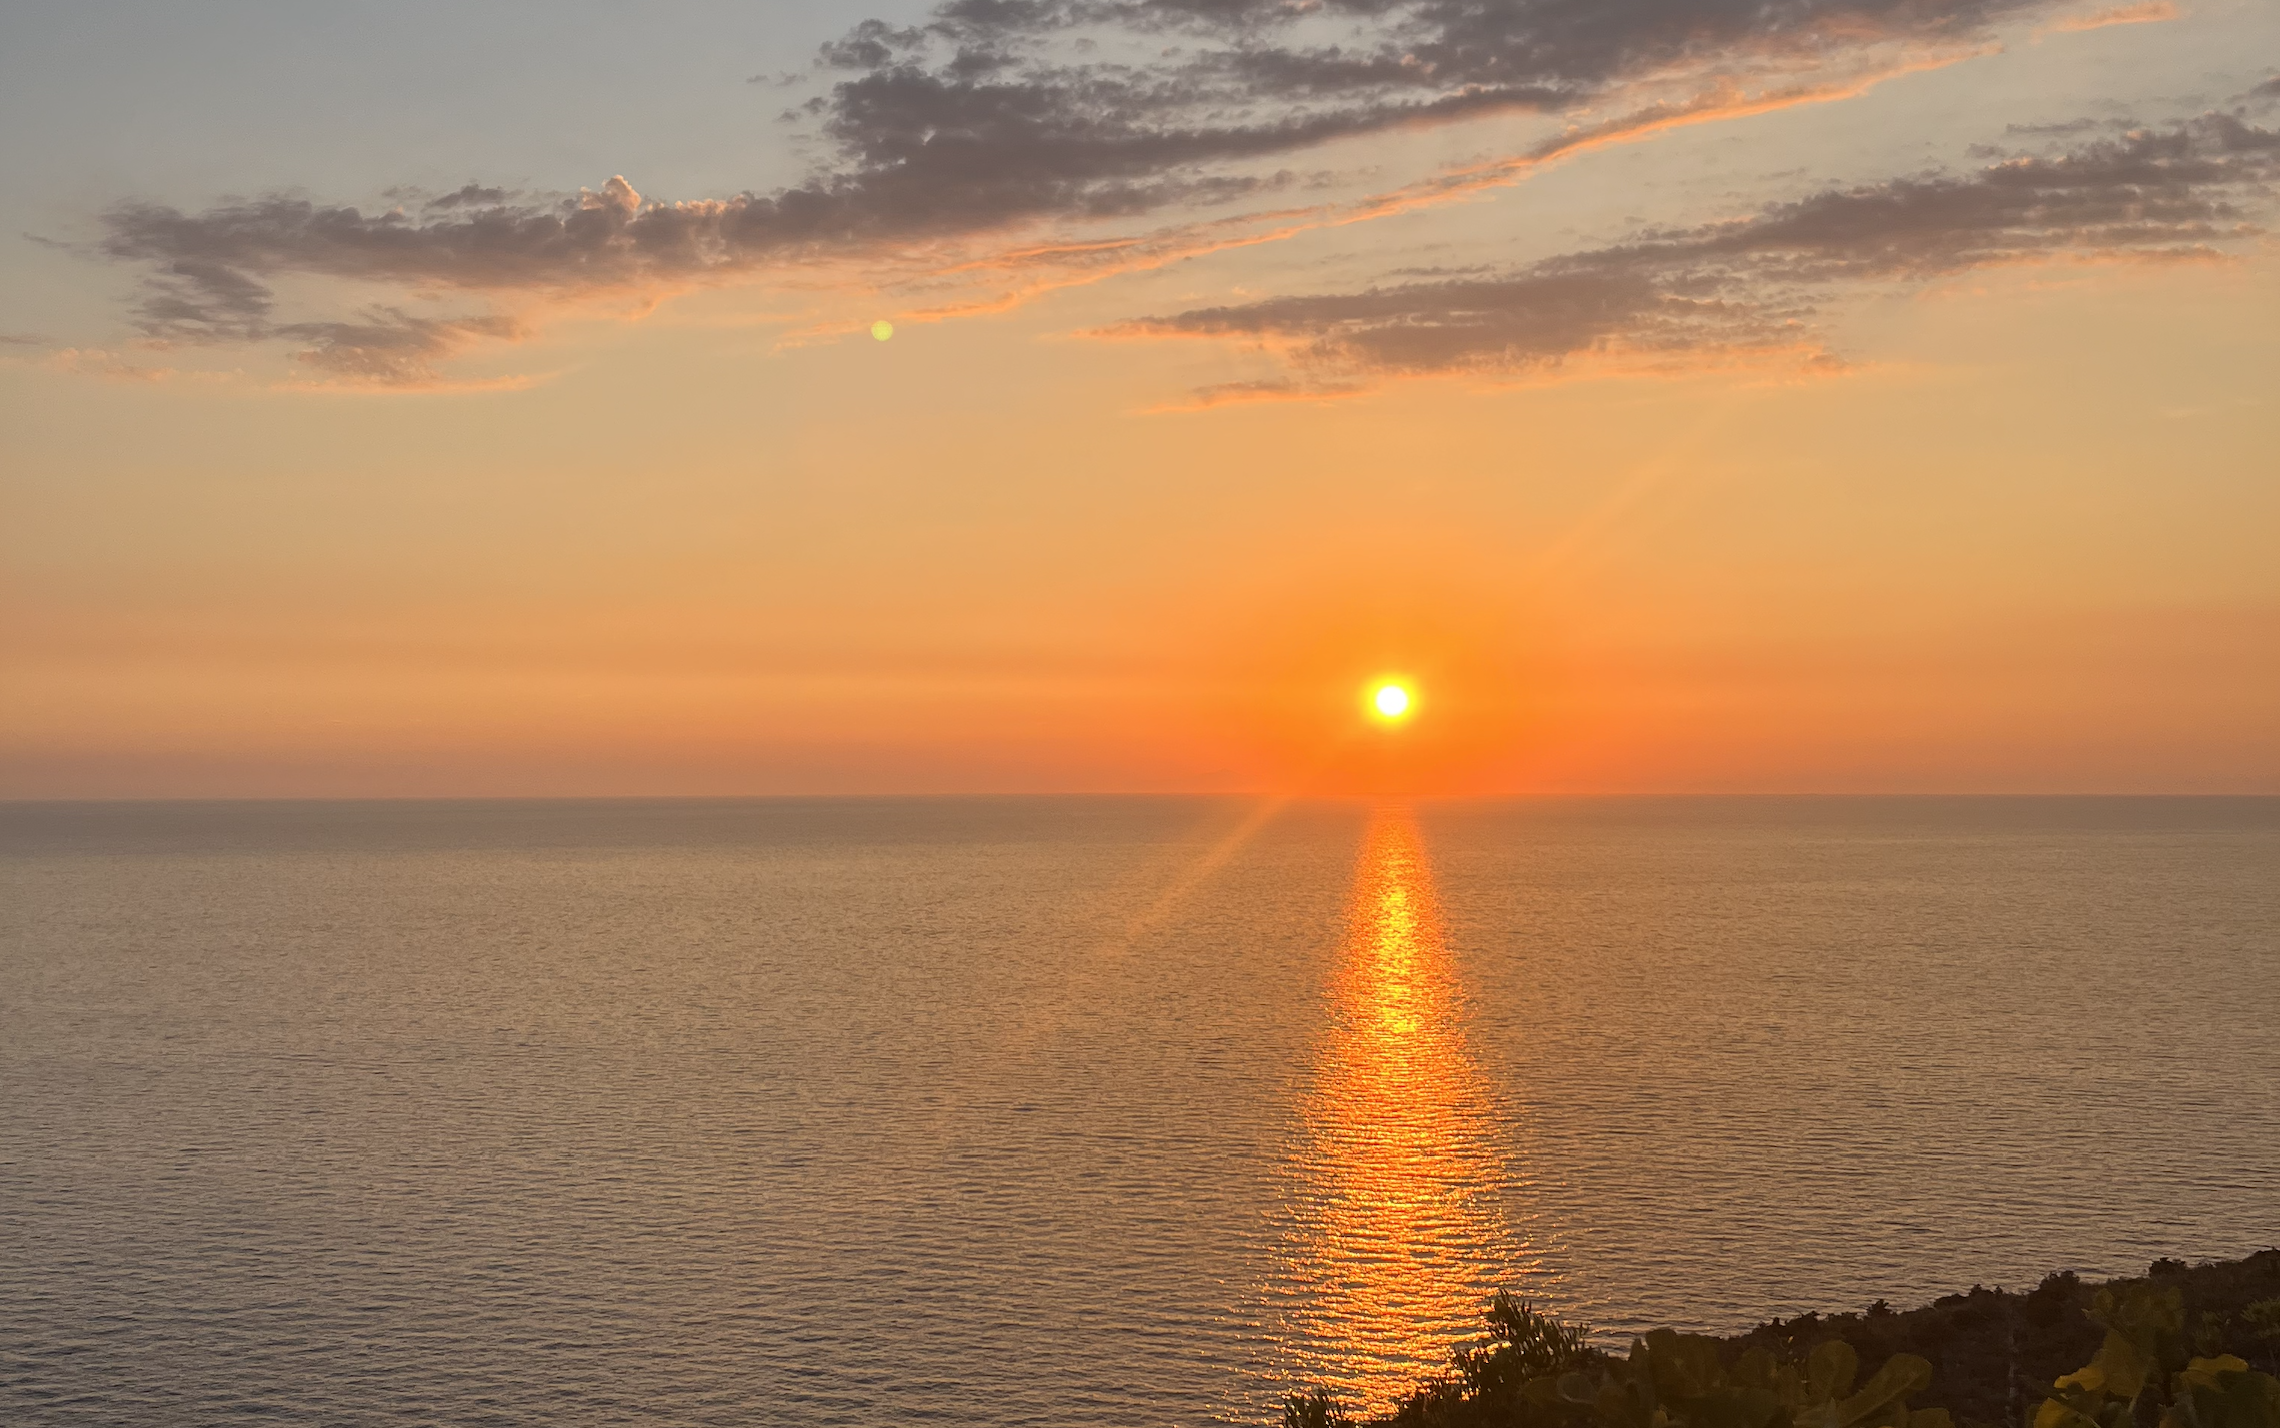
\includegraphics[width=0.6\linewidth]{Screenshot 2025-07-14 at 19.09.27.png}
    \label{fig:enter-label}
\end{figure}
\end{frame}

\begin{frame}{Extra: Functional inequalities}

    \begin{block}{Theorem}
Let $K$ be an irreducible and reversible Markov kernel on a finite set $\X$ with $\Ric_K\ge \kappa$ or $\Ric\ge \lambda >0$. The following inequalities hold:
\begin{align}
  \tag{HWI($\kappa$)}
  \cH(\rho)~\le~\W(\rho,\mathbf{1})\sqrt{\mathcal{I}(\rho)}-\frac{\kappa}{2}\W(\rho,\mathbf{1})^2
\end{align}
\vspace{-25pt}

\begin{align}
  \tag{MLSI($\lambda$)}
  \label{eq:ModLSI}
    \cH(\rho)~\le~\frac{1}{2\lambda}\mathcal{I}(\rho)
\end{align}
\vspace{-20pt}
  \begin{align}
    \tag{T$_\W$($\lambda$)}
  \label{eq:Tal}
      \W(\rho,\mathbf{1})~\le~\sqrt{\frac{2}{\lambda}\cH(\rho)}
  \end{align}


  \begin{align}
    \tag{{P($\lambda$)}}
  \label{eq:Poinc}
         ||\varphi||^2_\pi~\le~
         \frac{1}{\lambda}||\nabla\varphi||^2_\pi
  \end{align}
holds for all functions $\psi : \X \to \R$.
\end{block}
\end{frame}

\end{document}